\chapter{Calorimeter commissioning}
\label{ch:commissioning}

%% a refaire

The commissioning of the SuperNEMO demonstrator has begun in $2019$ and data were taken with the whole calorimeter

By the end of the year $2020$, the SuperNEMO demonstrator will be encapsulated in an anti radon tent.
The patch panel will insure passage of cables from the inside, to the outside of the anti radon tent, therefore doubling the amount of cables needed for the calorimeter.
The check of every cable condition is mandatory to control and eventually fix them.

The first two sections describe the start-up of the calorimeter, with the first data acquisitions and the various calibration operations that have been carried out by the collaboration.
The rest of the chapter deals with the work done within the framework of this PhD in order to verify the operating state of the calorimeter and its cables, after integration.


\section{Optical modules calibration}

It is necessary to check the correct operation of the whole calorimeter as well as each individual optical module, in order to repair and correct it if necessary.

\subsection{Pulse shape studies}

It is interesting to study the shape of the pulses sampled by the electronic boards, as it allows the identification of the presence of pre- or post-pulses that may be caused by undesired interactions, such as contamination of photomultipliers' vacuum by Helium, or the interaction of photons from the laboratory lighting, due to defects in the detector's light tightness.
A study performed by William Queen, a PhD student at UCL, allowed to determine a reference model for the expected shape of calorimeter waveforms.
An example of an awaited waveform is given in fig.~\ref{fig:waveform}.
\begin{figure}[h!]
  \centering
  \includegraphics[width=1\textwidth]{commissioning/fig_commissioning/waveform.pdf}
  \caption{Calorimeter waveform visualisation with the SNFee software.
    \label{fig:waveform}}
\end{figure}
The pulses received by the calorimeter can then be compared with this standard waveform, allowing any issues to be detected and resolved.



\subsection{Baseline studies}

The baseline is the part of the signal that is before the signal pulse.
Slight signal fluctuations can be observed in this area due to electronic noise, for example.
By averaging the amplitude value in this area, a reference can be defined to calculate the pulse amplitude.
This average is calculated by default directly by the calorimeter front-end boards, over the first $6.25$ nanoseconds of the signal.
In order to minimise the impact of statistical fluctuations on the baseline calculation, a more efficient analysis has been developed by Hichem Tedjditi, a PhD student at the CPPM, allowing to calculate it over an extended time.
The calculation of this average starts at the opening of the acquisition window, up to the rising edge of the signal pulse, which is detected automatically.
The presence of pre-pulses is also automatically characterised.
This analysis is done off-line and participates in the verification of the optical modules condition, after the installation of the calorimeter, and throughout the data acquisition of the demonstrator.

\subsection{Gain studies}


When a particle deposits energy as it interacts in the scintillator, the detection chain that follows enables a quantity of charge to be recovered at the PM voltage divider, that is proportional to the first energy deposited and depends on the high voltage applied to the photomultipliers.
In the SuperNEMO detector, these voltages can be adjusted individually for each block.
Charge and amplitude spectra can be obtained for each optical module and therefore depend on the high voltage applied.
As the optical modules are triggered from a signal amplitude threshold, it is necessary that the gains of all the optical modules of the calorimeter are equalised, in order to have comparable threshold values.
For the SuperNEMO calorimeter, this value has been set at an amplitude of $200$~mV for $1$~MeV deposited, corresponding to a $612$~mV gain.
Each optical module has then to be calibrated after installation, in order to reach this standard value and equalise all the PM responses.
The current study has been led by Axel Pin, a PhD student from CENBG.

This calibration consist in the optical module gains alignment, by obtaining a new high voltage value to be applied from the amplitude spectrum.
To determine the current gain of an optical module, one must first obtain its amplitude (or charge) spectrum and then locate a particular point on this spectrum.
To obtain these spectra, long runs (few hours) have been taken with the demonstrator, without the $^{207}$Bi calibration sources.
For this study, the chosen point is located at the end of the spectrum, where the only contribution of Thallium is expected in the $2e$ channel.
Once this gain is obtained, a reference gain is computed using simulations of \Tl\ decays inside the source foils.
The same particular point is determined, which corresponds to a given energy (as simulations allow to construct energy spectra).
Therefore, two gains are obtained one for real data and the other for simulations, allowing to determine the optimal high voltage value to apply for each photomultiplier.
The gains distributions before and after equalisation are presented in Fig.~\ref{fig:gain}.
\\...\\
The gain adjustment method have been effective as the distribution mean stands at $606.5\pm1.4$~mV at $3$~MeV, $8$~\% FWHM.

Now the optimal high voltages have been determined for each optical module, the collaboration will have to monitor the their gain, in order to insure the stability of the SuperNEMO calorimeter.

%% Depending on the value of this voltage, the gain $G_{OM}$ expected for a given optical module vary as:
%% \begin{equation}
%% G_{OM}=KV^{N\alpha}\,,
%% \end{equation}
%% where $K$ is a proportionality constant, $V$ is the high voltage applied to the photomultiplier, $N$ the number of dynodes and $\alpha$ is a coefficient depending on the PM characteristics.


\subsection{Energy calibration}
\label{sec:comm_energy_calibration}

As described in Sec.~\ref{subsec:OMtimeResponse}, the collected charge at photomultiplier voltage divider is proportional to the amount of incident photoelectrons, thus to the initially deposited energy inside the scintillator.
Once optical modules were assembled (optical coupling, packing, shielding integration), they were individually tested at Bordeaux laboratory, CENBG, with an electron spectrometer~\cite{HuberThesis}.
Their energy resolutions for $1$ MeV-electrons at the centre of scintillator front face were determined.
For optical modules assembled with $8$'' photomultipliers, it is in average of $8.19$\%.

Supply high voltages were characterised and set individually for each optical module to their to optimal values.
However, after the calorimeter integration, due to possible modifications of optical module characteristics, amplitude spectra of each optical block have to be re-aligned.
This work was also performed by Axel Pin, PhD student at CENBG.
We give in this section a summary of this energy calibration study.

The energy calibration method consists to find a particular point of a charge or amplitude spectrum, the Compton edge of \Tl\ for this study.
Looking for the same location on simulated \Tl\ energy spectra, a charge-energy or amplitude-energy correspondence can be made and applied to calibrate each optical module in energy.
In Fig.~\ref{fig:} are displayed the charge spectrum for $8$'' optical modules before energy calibration, as well as the energy spectrum after the calibration factor have been applied.
\\...\\
The distribution width is greatly improved by the energy calibration, going from $22.5$\%~FWHM to $3.9$\%~FWHM.

I also performed another energy calibration using the data acquisition and simulations with a Cobalt source, using the Cobalt peak at $1$~MeV.
This is discussed in Chapter~\ref{ch:Cobalt_study}.


\section{Light Injection System}
\label{sec:LI}

The LIS is a calibration method sending light pulses in optical modules for energy calibration purposes.
It has been detailed in Chapter~\ref{ch:detector}.

In the framework of this PhD, I took part in the analysis of the first commissioning data taken with this system.
All results presented in this sub-section are currently being improved by the collaboration.
In Fig.~\ref{fig:LI_counts} is displayed the simulated light intensity received by each optical module of the French main wall, for a data acquisition of $\sim20$~minutes with all LEDs.
\begin{figure}[h!]
  \centering
  \includegraphics[width=15cm]{commissioning/fig_commissioning/LI_1d_counts.pdf}
  \caption{Quantity of light received by each OM (labelled with OM index) of the French main wall.
    Each coloured marker represents counting rates for one area of the detector, that is to say one group of optical modules lighted by the same LED.
    The area $1$ (dark red dots) is not receiving light from its corresponding LED.
    \label{fig:LI_counts}}
\end{figure}
A total of $20$ LEDs allow to calibrate all optical modules of the two main walls, the X-Walls and $\gamma$-vetos.
Optical modules on the same main wall are divided into $5$ distinct groups, each illuminated via optical fibers by the light of one LED.
In the figure each of the $5$ area is represented.
Optical modules from area $1$ do not receive light from their associated LED, denoting a possible connection problem at the bundle (all fibers coming from one LED are grouped together in one bundle before being distributed on the calorimeter wall), or an issue with the LED itself.
It has been determined that this issue is intermittent, and sometimes affect other areas, possibly showing a more general problem related to the power supply of the LEDs.
This issue does not seem to be serious and is currently under investigation.

After checking the LED operation and quantity of light received, the amplitude spectra for each area have been studied and are presented in Fig.~\ref{fig:LI_ampl}.
\begin{figure}[h!]
  \centering
  \includegraphics[width=15cm]{commissioning/fig_commissioning/LI_mean_ampl.pdf}
  \caption{The mean signal amplitude distribution for each optical module is presented.
    One colour stands for one area of the half detector.
    In Grey is the total mean amplitude distribution.
    \label{fig:LI_ampl}}
\end{figure}
These spectra are very discontinuous and above all very spread out in amplitude.
The fact that the distributions are wide is not surprising, as the amount of light received by an optical module depends on many parameters, such as the location of the optical fibre in the bundle, which determines how close the fibre is to the LED.
The angle at which the optical fibre enters the scintillator can also greatly influence this quantity.
But the potentially worrying thing is that the amplitudes can go up to very high values.
In practice, the acquisition does not record signal amplitudes above a few hundred mV.
When the amplitude is too large, the signal is just truncated.
It is then the SNFee off-line analysis code which, when trying to determine the location of the waveform peak, performs an extrapolation and gives such large amplitudes.
So even if these values do not correspond to the actual amount of light received by the optical modules, the amplitude is still too high compared to what is expected.
Calibration operations are underway to harmonise this quantity.

In the following, the work I achieve on the calorimeter commissioning is discuss in detail.


\section{Calorimeter cabling network}
\label{sec:reflecto}

In this section is presented an analysis performed in order to check the status of calorimeter signal cables.
I was involved in most of the stages of the detector cabling, from cutting the calorimeter signal cables at LAL, to their installation in Modane on the various walls of the calorimeter, via their welding to the PM voltage dividers and their organisation on the patch panel.
Although not covered in this analysis, I was also involved in the connection (under the detector) of the tracker cables and their routing from the detector to the electronics.
These steps were crucial and gave me a good knowledge of the detector I am working on.

\subsection{Motivations}

The cabling network of SuperNEMO is described in detail in Chapter~\ref{ch:detector}.
In particular, the calorimeter is segmented in $712$ optical modules, each connected to the electronics by the photomultiplier divider throught $2$ cables.
The first one provides the high voltage (HV) necessary for its operation.
The other one, the so-called signal cable, is a coaxial cable collecting and transporting the charge corresponding to the optical module signal.
Regarding only the last category, $1424$ coaxial cables were cut, assembled, connector-mounted, transported and installed at LSM\footnote{$712$ optical modules are connected to the electronics through two signal cables, one internal and one external, linked at patch panel.}.

Each coaxial cable length was determined by taking into account the demonstrator design.
All external coaxial cables were designed to be $7$ meters-long -- the distance between electronic boards and patch panel being the same for all channels -- and internal cable lengths have been adapted to fit the distance from the patch panel to each optical module.
Cutting and labelling all cables lasted several weeks.
After all cables were transported and installed at LSM, we have to check each coaxial cable condition, for several reasons:
\begin{itemize*}
\item make sure that cables have not been damaged during the transport and the installation,
\item control if no swap between internal cables has been made during cable labelling or calorimeter cabling,
\item check if the coaxial cables were cut at right lengths,
\item estimate time delays induced by the signal transit time inside the coaxial cables.
\end{itemize*}
The last point is essential: knowing that the  electron velocity in a coaxial cable is a determined constant value, the longer the cable, the longer it takes for the signal to reach the electronics.
As coaxial cables have different lengths, this transit time could delay the signal transmission and therefore bias the calorimeter time-of-flight measurements.
Therefore, each coaxial cable length has to be characterised, and the transit time has to be stored in a database made available to the collaboration.
This last aspect is of major importance, especially for time coincidences studies using particle time-of-flights.

\subsection{Experimental setup}

In order to control each cable status, we used a feature provided by SuperNEMO's electronics, where an electrical signal, called \emph{primary} pulse, is generated by the calorimeter front-end boards and sent to each channel.
The Fig.~\ref{fig:reflecto_scheme} summarises the three possible scenarios when such a pulse is sent in the SuperNEMO calorimeter cables.
\begin{figure}[h!]
  \centering
  \begin{subfigure}[b]{0.3\textwidth}
    \centering
    \includegraphics[width=1.1\textwidth]{commissioning/fig_commissioning/scheme_reflecto.pdf}
    \captionsetup{justification=centering}
    \caption{Normal reflection at PM divider.
      \label{subfig:reflecto_normal}}
  \end{subfigure}
  \hfill
  \begin{subfigure}[b]{0.3\textwidth}
    \centering
    \includegraphics[width=1.1\textwidth]{commissioning/fig_commissioning/scheme_reflecto_1.pdf}
    \captionsetup{justification=centering}
    \caption{Cable not connected at PM.
      \label{subfig:reflecto_pmt}}
  \end{subfigure}
  \hfill
  \begin{subfigure}[b]{0.3\textwidth}
    \centering
    \includegraphics[width=1.1\textwidth]{commissioning/fig_commissioning/scheme_reflecto_2.pdf}
    \captionsetup{justification=centering}
    \caption{Cable not connected at patch panel.
      \label{subfig:reflecto_pp}}
  \end{subfigure}
  \caption{Three possible scenarios occuring when a signal is sent in the SuperNEMO coaxial cables.
    The electronic boards are symbolised by black chips, and the patch panel by red vertical bars.
    The coaxial cable, pictured by horizontal lines, connects the electonics to the PM divider.
    (a) The cable is well connected at the patch panel and at the PM. The signal reflects at the PM divider.
    (b) The cable is not connected (or badly connected) at the PM divider. The signal is reflected at the end of the internal cable.
    (c) The cable is not connected (or badly connected) at patch panel. The signal is reflected at the end of the external cable.
    \label{fig:reflecto_scheme}}
\end{figure}
\begin{itemize}
\item Fig.~\ref{subfig:reflecto_normal}: under normal cable operating conditions, the pulse travels along the coaxial cable until it reaches the photomultiplier.
\item Fig.~\ref{subfig:reflecto_pmt}: it may happen a cable was not (or badly) connected to the PM divider.
  In that case the signal reflects at the end of the internal cable.
  This scenario is addressed in Sec.~\ref{subsec:pulse_shape}.
\item Fig.~\ref{subfig:reflecto_pp}: if the cable is not connected, or misconnected, at the patch panel level, the signal undergoes a reflection at the end of the external cable.
  This scenario is addressed in Sec.~\ref{subsec:timing}.
\end{itemize}
In all three cases, the signal comes back to the electronics where it is recorded, after a more or less long cable distance.
This return pulse is naturally called \emph{secondary} pulse.

An example of a normal set of primary and secondary pulses, under normal cable operating conditions, is displayed in Fig.~\ref{fig:total_waveform}.
\begin{figure}[h!]
  \centering
  \includegraphics[width=1\textwidth]{commissioning/fig_commissioning/pulses_example.pdf}
  \caption{Primary (left) and secondary (right) pulses for different cable lengths under normal cable operating conditions.
    Such pulse shapes are used as a reference to detect anormal pulses and thus identify possible defaults.
    \label{fig:total_waveform}}
\end{figure}
All primary pulses are sent almost simultaneously inside different electronic channels, so they appear all superimposed.
Depending on the cable length they travelled through, secondary pulses return to the electronics with more or less delay.

In order to accumulate enough statistics, we send thousands of pulses in each coaxial cable.
The analyses of the shape and of the arrival time of those secondary pulses for each channel is called \emph{reflectometry}, and allow us to check the coaxial cable conditions and to control their lengths.

Comment les pulses vont être affectés: mettre pulse shape analysis avant.
Certains pb déco élec résolus
Called reflecto

\subsection{Pulse timing: controlling cable lengths}
\label{subsec:timing}

The first step of this analysis is to experimentally determine the length $l_{j}^{m}$ for all signal cables $j$ installed on the demonstrator.
This length is defined as
\begin{equation}
  l_{j}^{m}= 0.5\,t_{j}\,v_{p}\, ,
\end{equation}
where $t_{j}$ stands as the time made by the electrons to do a round trip between one electronic channel and one PM, and $v_{p}$ is the velocity of electrons in the coaxial cables, which can be expressed as a fraction of light speed in vacuum, $c$.
The time difference $t_{j}$ between the primary pulse and the secondary pulse is written as
\begin{equation}
  t_{j} = \braket{t_{\text{secondary pulse}}-t_{\text{primary pulse}}}_{p} \, \text{,}
\end{equation}
$\braket{}_{p}$ being the average over all pulses sent in one single cable $j$.
The velocity $v_{p}$ is supplied by the cable manufacturer as
\begin{equation*}
  v_{p}=\frac{c}{\sqrt{\epsilon_{r}}}\,\text{,}
\end{equation*}
with $\epsilon_{r}$ the relative dielectric constant of the material.
Therefore, this celerity depends on the components.
For the coaxial cables chosen in the demonstrator design, the data sheet of the cable gives ${v_{p}=0.69\,c}$.
A study is performed to verify experimentally the value of $v_{p}$.
Three cables of different lengths are measured with a precision of $1$ cm.
A thousand of primary pulses are sent in each of the three cables, then the time for each secondary pulse is recorded.
At the end, we have three independent measures of the velocity $v_{p}$ in the used coaxial cables.
In Fig.~\ref{fig:celerity} is displayed the lengths $l_{j}$ as a function of the times $t_{j}$.
\begin{figure}[h!]
  \centering
  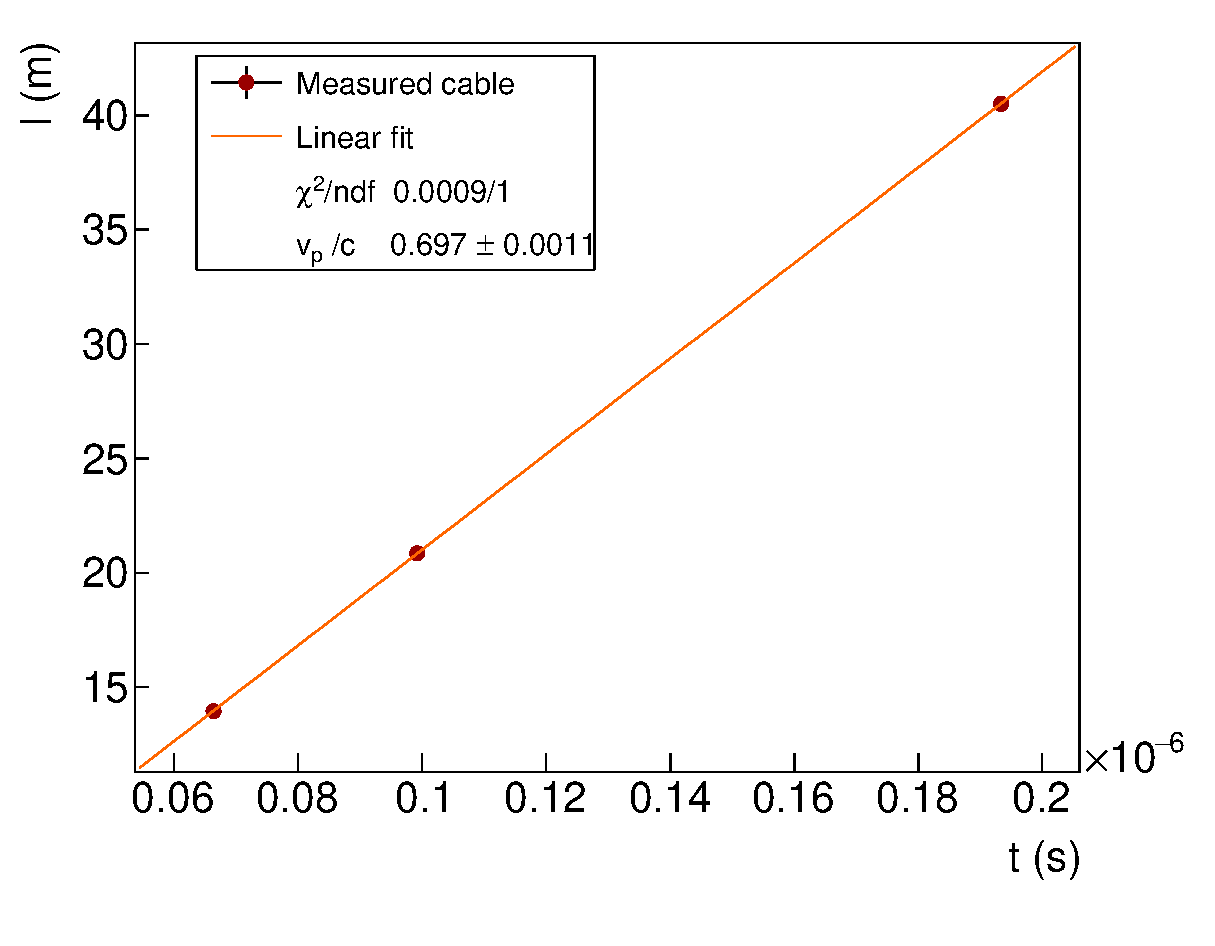
\includegraphics[width=15cm]{commissioning/fig_commissioning/celerity.eps}
  \caption{Three different lengths $l_{j}$ of cables are measured.
    Pulses are sent inside all cables.
    The lengths $l_{j}$ are plotted as a function of the time differences $t_{j}$ between primary and secondary pulses.
    The value of $v_{p}/c$ fitted from the data points is displayed.
    This value of $0.697\pm 0.0011$ shows the compatibility with the one supplied by the constructor, of $0.69$ c.
    \label{fig:celerity}}
\end{figure}
The fitted value of $v_{p}/c = 0.697\pm 0.0011$ is displayed and shows a compatibility up to $7\sigma$ with the data sheet.

As we want to determine the time interval $t_{j}$, we have to define what is the \emph{time} of a pulse.
In this analysis, we use a technique called Constant Fraction Discriminator (CFD), providing an amplitude-independent information about time of a pulse.
This algorithm aims at tracking a signal and defining its time arrival at a given fraction $f$ of its maximal amplitude.
The two main advantages of this technique is that it provides an efficient rejection of the noise in the acquisition window, and gives a good resolution on the measured time.
Nevertheless, the possible influence of the chosen value for the $f$ parameter on this time resolution has to be investigated.
We perform such a study in Sec.~\ref{subsec:CFD}.
We concluded that the highest precision on the time measurement arises for $f = 40\%$, and we adopt this value for the following analysis.
A graphic representation of the CFD time search is given in fig.~\ref{fig:CFD}.
\begin{figure}[h!]
  \centering
  \includegraphics[trim={1.2cm 1.5cm 1.7cm 3.1cm},clip,width=1\textwidth]{commissioning/fig_commissioning/CFD_example_zoom.pdf}
  \caption{ Zoom on the secondary pulse.
    A representation of time computed with a Constant Fraction Discriminator (CFD) is provided.
    Its maximal amplitude (red dotted line) and its fraction for $\text{f}=40\%$ (green dotted line) are displayed.
    The time $\text{T}_{\text{pulse}}$ (orange dotted line) represents the time of arrival of the secondary pulse computed with CFD, with the fraction $\text{f}=40\%$.
    \label{fig:CFD}}
\end{figure}
As we want to measure the installed cable lengths $l^{m}_{j}$, and compare them to the initially designed ones, $l^{d}_{j}$, we define the length difference $\Delta L_{j}$ as:
\begin{equation}
  \Delta L_{j} = l^{m}_{j}-l^{d}_{j}\, .
\end{equation}
In Fig.~\ref{fig:LengthDiff} is displayed the distribution $\Delta L$ for all the measured lengths.
\begin{figure}[h!]
  \centering
  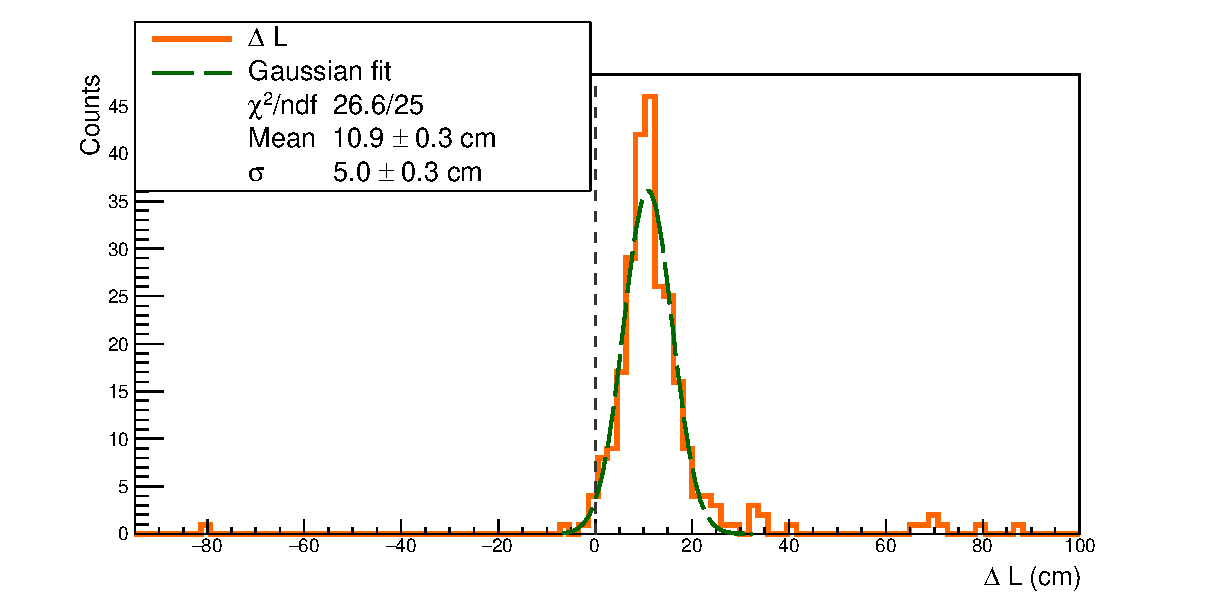
\includegraphics[width=15cm]{commissioning/fig_commissioning/length_diff.eps}

  \caption{The distribution of difference between the measured lengths $l^{m}$ and the expected lengths $l^{d}$ is displayed in orange solid line.
    The black dashed line represents the case where $l^{m}_{j} = l^{d}_{j} \;\forall j$.
    The Gaussian fit (green dashed line) presents a mean of $10.9 \pm 0.3$ cm.
    Some data points considered as outliers are beyond $3\sigma$.
    \label{fig:LengthDiff}}
\end{figure}
In hypothetical perfect conditions, all the cables should fit the design length, in other words, $l^{d}_{j} = l^{m}_{j}$.
Consequently the $\Delta L$ distribution should a peak at zero, as materialised by the black dashed line.
However, in real conditions, the measured length can be different from the designed one, leading the $\Delta L$ distribution plotted in orange solid line.
We conclude that the observed cable length $l^{m}$ differs from $l^{d}$ by $+10.9\pm 0.3$ cm, meaning that cables are longer than expected in average.
This may reveal a bias coming from the device used to cut the cables.
In fact, during cable cutting work, we noticed that the cutting device had a tendency to slip, probably leading to cables with extra lengths.
We assumed the cutting device has a given probability to slip for one meter of cable.
If this is the case, the probability for the device to give extra length should increase with the cable length.

To verify this assumption, we plot in Fig.~\ref{fig:CutBias} the length difference $\Delta L$ as a function of the initial design length $l^{d}$ (cyan).
From those data points, we compute a linear fit (orange solid line), parameterised as $y = \alpha x + \beta$, revealing that the cutting device presents two different biases.
\begin{figure}[h!]
  \centering
  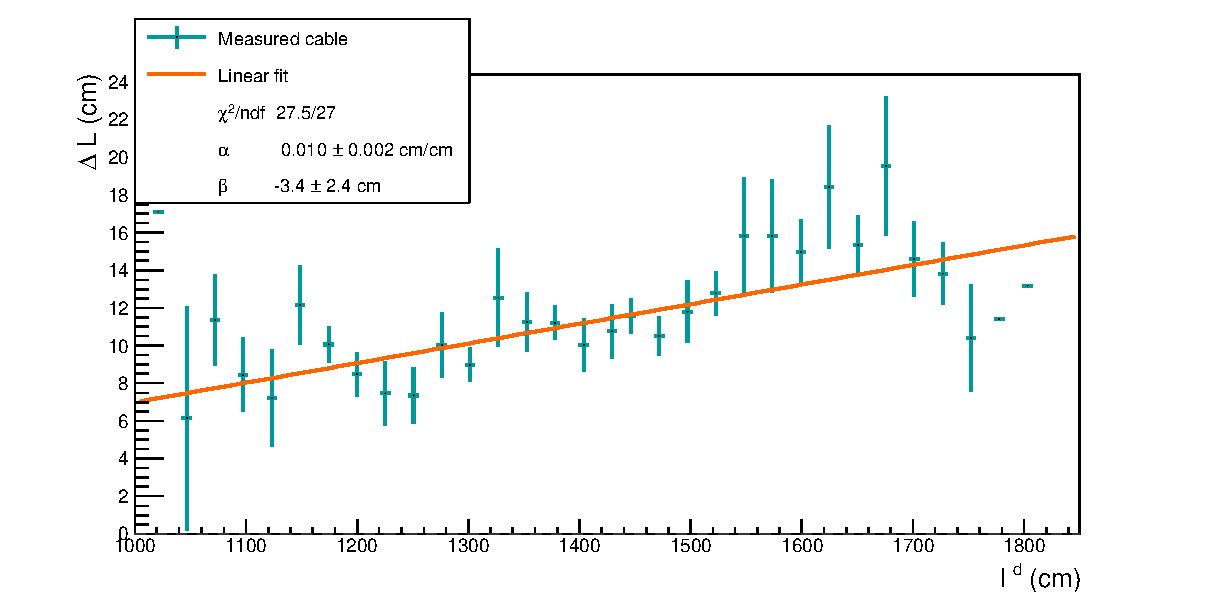
\includegraphics[width=15cm]{commissioning/fig_commissioning/cut_biais.eps}

  \caption{$\Delta L$ is plotted with $l^{d}$ (cyan), where $l^{d}$ is averaged for all the lengths designed to have the same value, being at the origin of vertical error bars.
    In black dashed line is represented the case where $l^{m} = l^{m}$.
    Data points are fitted by $\alpha x + \beta$, with $\alpha > 0$ and $\beta < 0$, revealing the two biases of the cutting device.
    \label{fig:CutBias}}
\end{figure}
The value of $\beta$ shows that the cutting device systematically took away $3.4$ cm of each cable.
Nevertheless, as the shortest cable was designed to be 10 meters long, there are no important consequences of this bias on the length difference $\Delta L$.
Besides, the slope $\alpha = 0.010\pm 0.002$ of the linear fit reveals that the cutting device adds one centimetre for every meter of cable, being compatible with the hypothesis on the cutting device sliding.
Hopefully this bias is not problematic as it makes most of the actual cable lengths longer than the design, while shorter lengths could have led to systematic connection issues to PMs.
However, we notice that a few cables have been cut too short by mistake, the worse of them being $80$ centimetres shorter than expected.
Fortunately, this cable  was successfully connected to PM despite this deficit.
On the contrary, few cables have a large extra length.
This probably is due to human punctual mistakes on top of the observed bias, but without any strong consequences for the calorimeter operation.
In conclusion, no important mistakes have been made when cutting cables, and we had no issue for connecting the only problematic cable.

If the main goal of this study is to check the lengths of coaxial cables, it also aims at correcting the time of recorded events, from the time made by the signal to travel from a PM to an electronic channel.
taking into account the time for the signal to travel through cables.
This become possible with the reflectometry study we performed.
Knowing real lengths of cables and using the celerity of the signal, we deduce the time needed for the signal to travel from one given PM divider to the electronic boards.
Then we can correct event times.

As explained previously, the time $t_{j}$ gives information about the length of the cable $j$.
We remind the coaxial cables are divided in two parts, one external and one internal, both linked by the so-called patch panel.
Thus we can use that travel time to detect possible disconnection of a cable at patch panel.
In fact, if one cable is not connected at the patch panel -- this case is illustrated in Fig.~\ref{subfig:reflecto_pp}, -- the pulse reflects at the end of the external cable part, going back to the electronic board.
This very short time, giving information about the location of the reflection, is used to tag a patch-panel disconnection.
Then, a simple check onsite can confirm this observation, and the external part of the cable can be connected to the patch panel.

This study allowed us to control and record the lengths of all coaxial cables installed on the SuperNEMO demonstrator at LSM, and gave information on the status of cable connections at patch panel.
We also have understood the main results on measured cable lengths and the functioning and biases of the cutting device that we used.

\subsection{Signal attenuation}
\label{subsec:attenuation}
The attenuation of an electric signal is a problem common to all electronic fields, and comes from the charge loss of an electromagnetic wave travelling in a medium.
%% Then, another test for controlling the cable condition is to check if this attenuation matches
%% the expectations (i.e. the attenuation per metre of cable given by constructor).
%% The signal attenuation car be define in two different ways:
%% \begin{itemize*}
%% \item using the signal amplitude ratio
%% \end{itemize*}
For a coaxial cable, this attenuation mainly depends on the signal frequency $f$ in MHz and on the cable characteristics.
For the coaxial cables, the theoretical linear attenuation $\alpha_{\text{att}}^{\text{th}}$, so be it the attenuation by metre of cable in dB/m, is supplied by the constructor as
\begin{equation}
  \alpha_{\text{att}}^{\text{th}} = f\sqrt{\epsilon}(\frac{a}{\sqrt{f}}+b)\,,
\end{equation}
where the factor $a$ depends on the diameter of the dielectric material on one side, and of the diameter of the conductor material on the other side, and where $b$ is function of the dielectric loss factor, characterising the material's dissipation of electromagnetic energy.
For the used coaxial cables, and with a frequency $f$ of few GHz for the signal pulses sent in cables, we calculate this attenuation as $\alpha_{\text{att}}^{\text{th}} = 1.22$ dB/m.
In a more general manner, the attenuation of a signal in dB is defined with the decimal logarithm of a power ratio.
We use this definition to determine the attenuation in the framework of the reflectometry analysis, defining the attenuation $\mathcal{A}$, for a given length of cable $l$, as
\begin{equation}
  \mathcal{A}=10\log_{10}\frac{V_{\text{primary pulse}}}{V_{\text{secondary pulse}}} \,\text{,}
\end{equation}
where $V_{i}$ is a quantity representing the intensity of the signal.
$V$ can correspond to the maximal amplitude of the pulse, as well as the \emph{integrated charge} of the pulse, defined as the amount of current received by the acquisition over a given time window.
As the provided data sheet does not specify the attenuation of which quantity (amplitude or charge) represents $\alpha_{\text{att}}^{\text{th}}$, we decide to investigate both in the following.
Then, we define the linear attenuation $\alpha_{\text{att}}^{\text{R}}$, measured by reflectometry in dB/m, with
\begin{equation}
  \mathcal{A} = f_{r}+\alpha_{\text{att}}^{\text{R}}\,l\,,
\end{equation}
with $f_{r} = -10\log_{10}R$, where $R$ is the reflection factor characterising the pulse reflection on the PM divider.
In fact, as the circuit is opened, the pulse is reflected at the PM divider, but only partially.
A part of the signal is not reflected but lost through the divider.
This reflection is characterised by $R$, which is function of the impedance $Z_{c}$ of the cable, and of the impedance $Z_{d}$ at the divider level, where the pulse is reflected.
It is written as
\begin{equation}
  R = \frac{Z_{d}-Z_{c}}{Z_{d}+Z_{c}}\,,
\end{equation}
where we have the limit
\begin{equation}
  \lim_{Z_{d} \to \infty} f_{r} = 0 \text{ and } R=1\,,
\end{equation}
expressing a total reflection occurring when the impedance at the PM divider is infinite.
The main goal here is to determine the value of $\alpha_{\text{att}}^{\text{R}}$, using the reflectometry data, and to compare it with $\alpha_{\text{att}}^{\text{th}}$.
Moreover, the impedance $Z_{d}$ value at PM divider can be estimated from the determination of $f_{r}$.
In Fig.~\ref{fig:attenuation} is shown the linear dependence between the attenuation $\mathcal{A}$ and the cable length $l$, and two data set are presented.
The cyan scattered markers represent the attenuation calculated from the amplitude ratio $A_{\text{primary pulse}}/A_{\text{secondary pulse}}$, and the magenta markers correspond to the attenuation calculated from the charge ratio $Q_{\text{primary pulse}}/Q_{\text{secondary pulse}}$.
The amplitude $A_{i}$ is given in mV and the charge $Q_{i}$ in mV.ns.
\begin{figure}[h!]
  \centering
  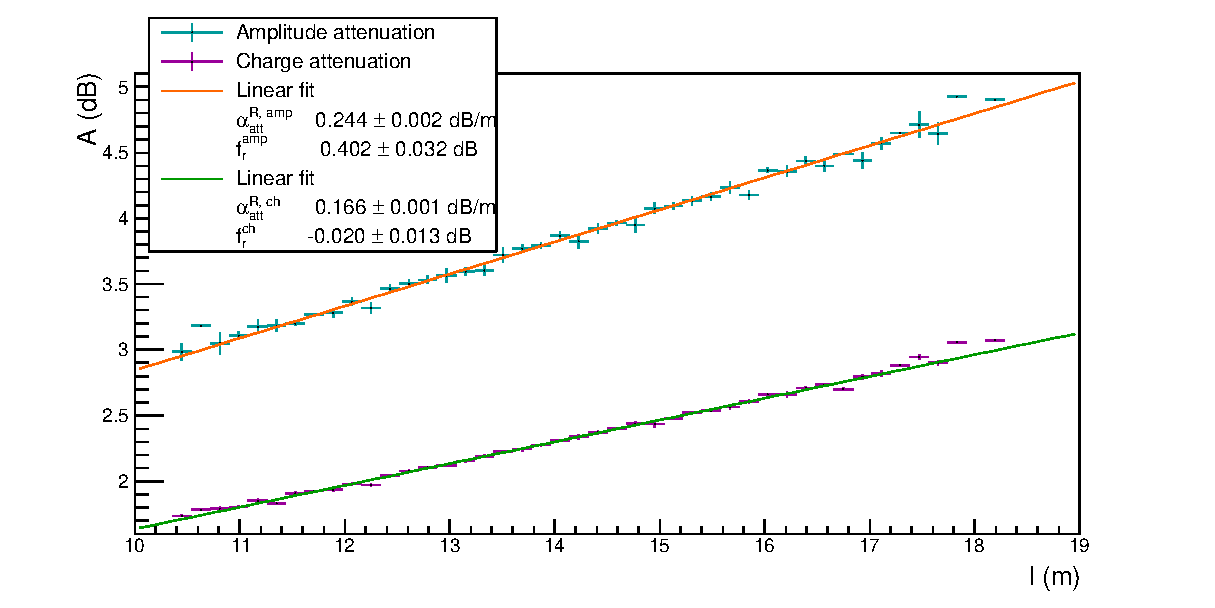
\includegraphics[width=15cm]{commissioning/fig_commissioning/attenuation_length.eps}
  \caption{The amplitude $\mathcal{A}$ is displayed as a function of the measured cable length $l$.
    The data set calculated with the amplitude (charge) is given in cyan (magenta) and fitted by a linear function in orange (green).
    The values of the slope, which represent the linear attenuation of the coaxial cables in dB/m, are respectively $\alpha_{\text{att}}^{\text{R, amp}} = 0.241\pm 0.000$dB/m and $\alpha_{\text{att}}^{\text{R, ch}} = 0.166\pm0.000$dB/m.
    The two $y$-intercept values, which represent the reflection of the pulse on the PM divider, are $f_{r}^{amp} = 0.402\pm 0.032$ dB and $f_{r}^{ch} = -0.020\pm 0.013$ dB.
    \label{fig:attenuation}}
\end{figure}
The values of $\alpha_{\text{att}}^{\text{R}}$ and $f_{r}$, for both amplitude and charge cases, are displayed in the legend.
Firstly, the two linear fits reveal that, whether calculated with the amplitude, or with the charge, the linear attenuation $\alpha_{\text{att}}^{\text{R}}$ is smaller than the calculated one $\alpha_{\text{att}}^{\text{th}}$ (for the amplitude case, $\alpha_{\text{att}}^{\text{th}}\simeq 5\times \alpha_{\text{att}}^{\text{R, amp}}$, and for the charge case $\alpha_{\text{att}}^{\text{th}}\simeq 7\times \alpha_{\text{att}}^{\text{R, ch}}$).
That means the signal is less affected, when transmitted by the cable, than expected.
Secondly, the attenuation in charge is less important that the attenuation in amplitude.
This can be easily explained: as it is integrated over time, the charge is a quantity less affected by amplitude variations that the amplitude itself.
For the same reason, the charge data set points are less spread than the amplitude ones, meaning that we are less sensitive to cable length variations when using the charge quantity.


This work achieved, we want to verify if no cable was damaged after installation.
Reflectometry also aimed at checking cable conditions by performing waveform shape analysis on secondary pulses.

\subsection{Pulse shape analysis}
\label{subsec:pulse_shape}
In Fig.~\ref{fig:CFD} is displayed an example of \emph{normal} pulse, which corresponds to the case represented in Fig.~\ref{subfig:reflecto_normal}.
In this case, the pulse sent in the cable travels to the PM, and goes back to the acquisition after reflection on the divider.


%% \subsection{Comparison with $^{60}$Co}

\subsection{Conclusion}
A faire : regarder le rising time en fonction de la longueur du cable
Regarder la différence de temps de montée du signal sur deux PMs très éloignés

%% \section{Calibrating the electronic boards}
%% \label{sec:TimeSynchroFEB}

%% \subsection{Principle}
%% \subsection{Measuring the time offset of front end boards}
%% \subsection{Results}


\section{Conclusion}
